\chapter{In Depth: Gaussian Mixture Models\label{Ch48}}
In particular, the nonprobabilistic nature of k-means and its use of simple
distance from cluster center to assign cluster membership leads to poor performance
for many real-world situations. Gaussian mixture models can be viewed as an extension of the ideas behind k-means, but can
also be a powerful tool for estimation beyond simple clustering.

An important observation for k-means is that these cluster models must be circular: k-means has no built-in way of accounting for oblong or elliptical clusters.

\begin{figure}
    \centering
    \begin{subfigure}[f]{.45\textwidth}
        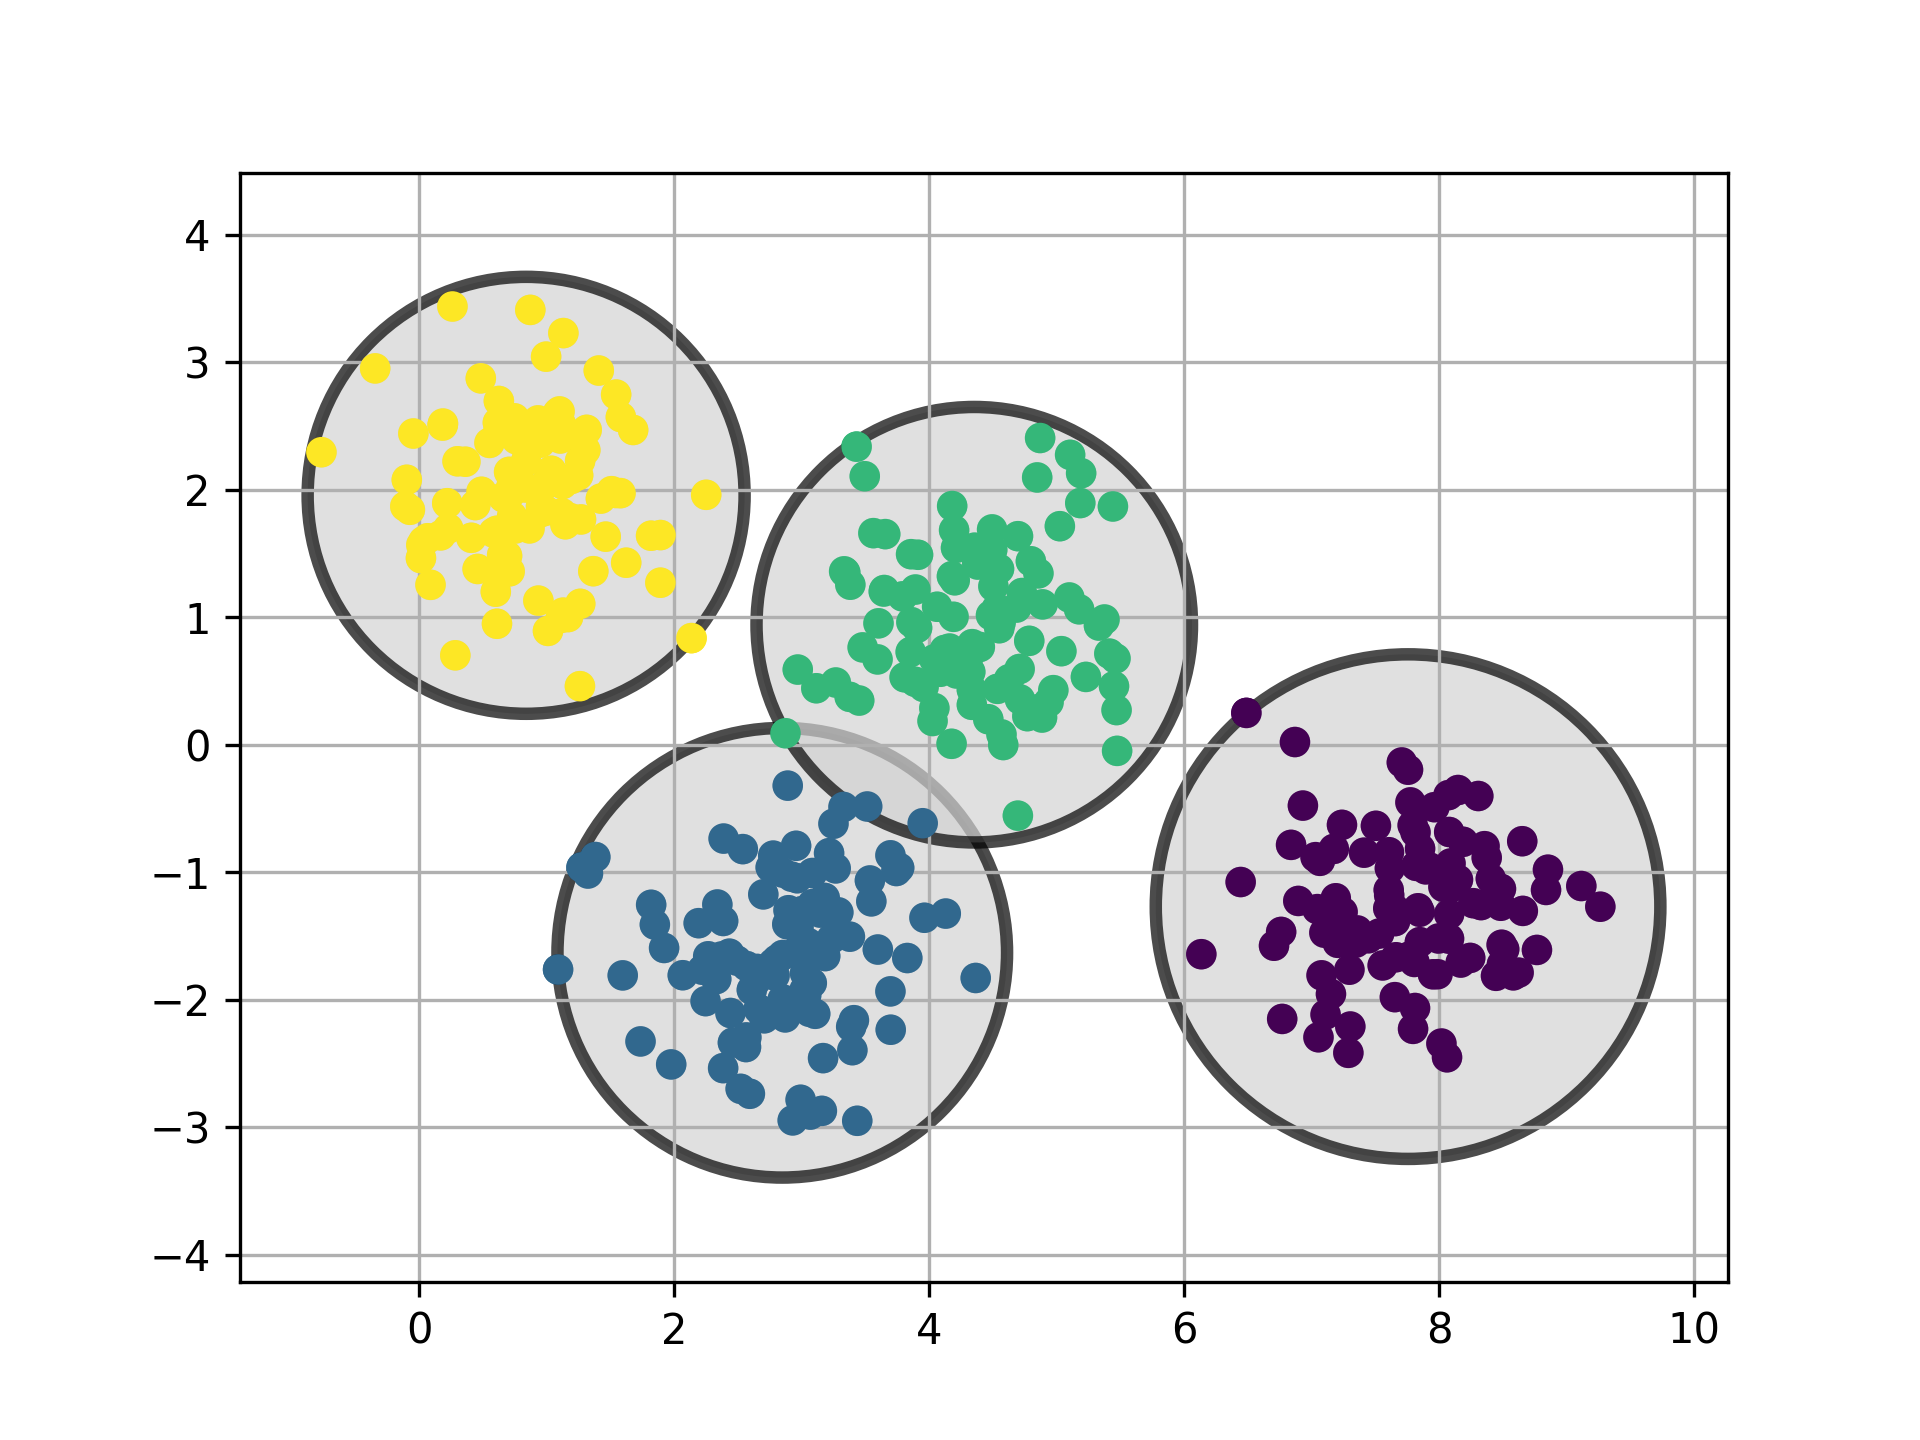
\includegraphics[width=\textwidth]{../img/fig48-2.png}
        \caption{The circular clusters implied by the k-means model}
    \end{subfigure}
    \hfill
    \begin{subfigure}[f]{.45\textwidth}
        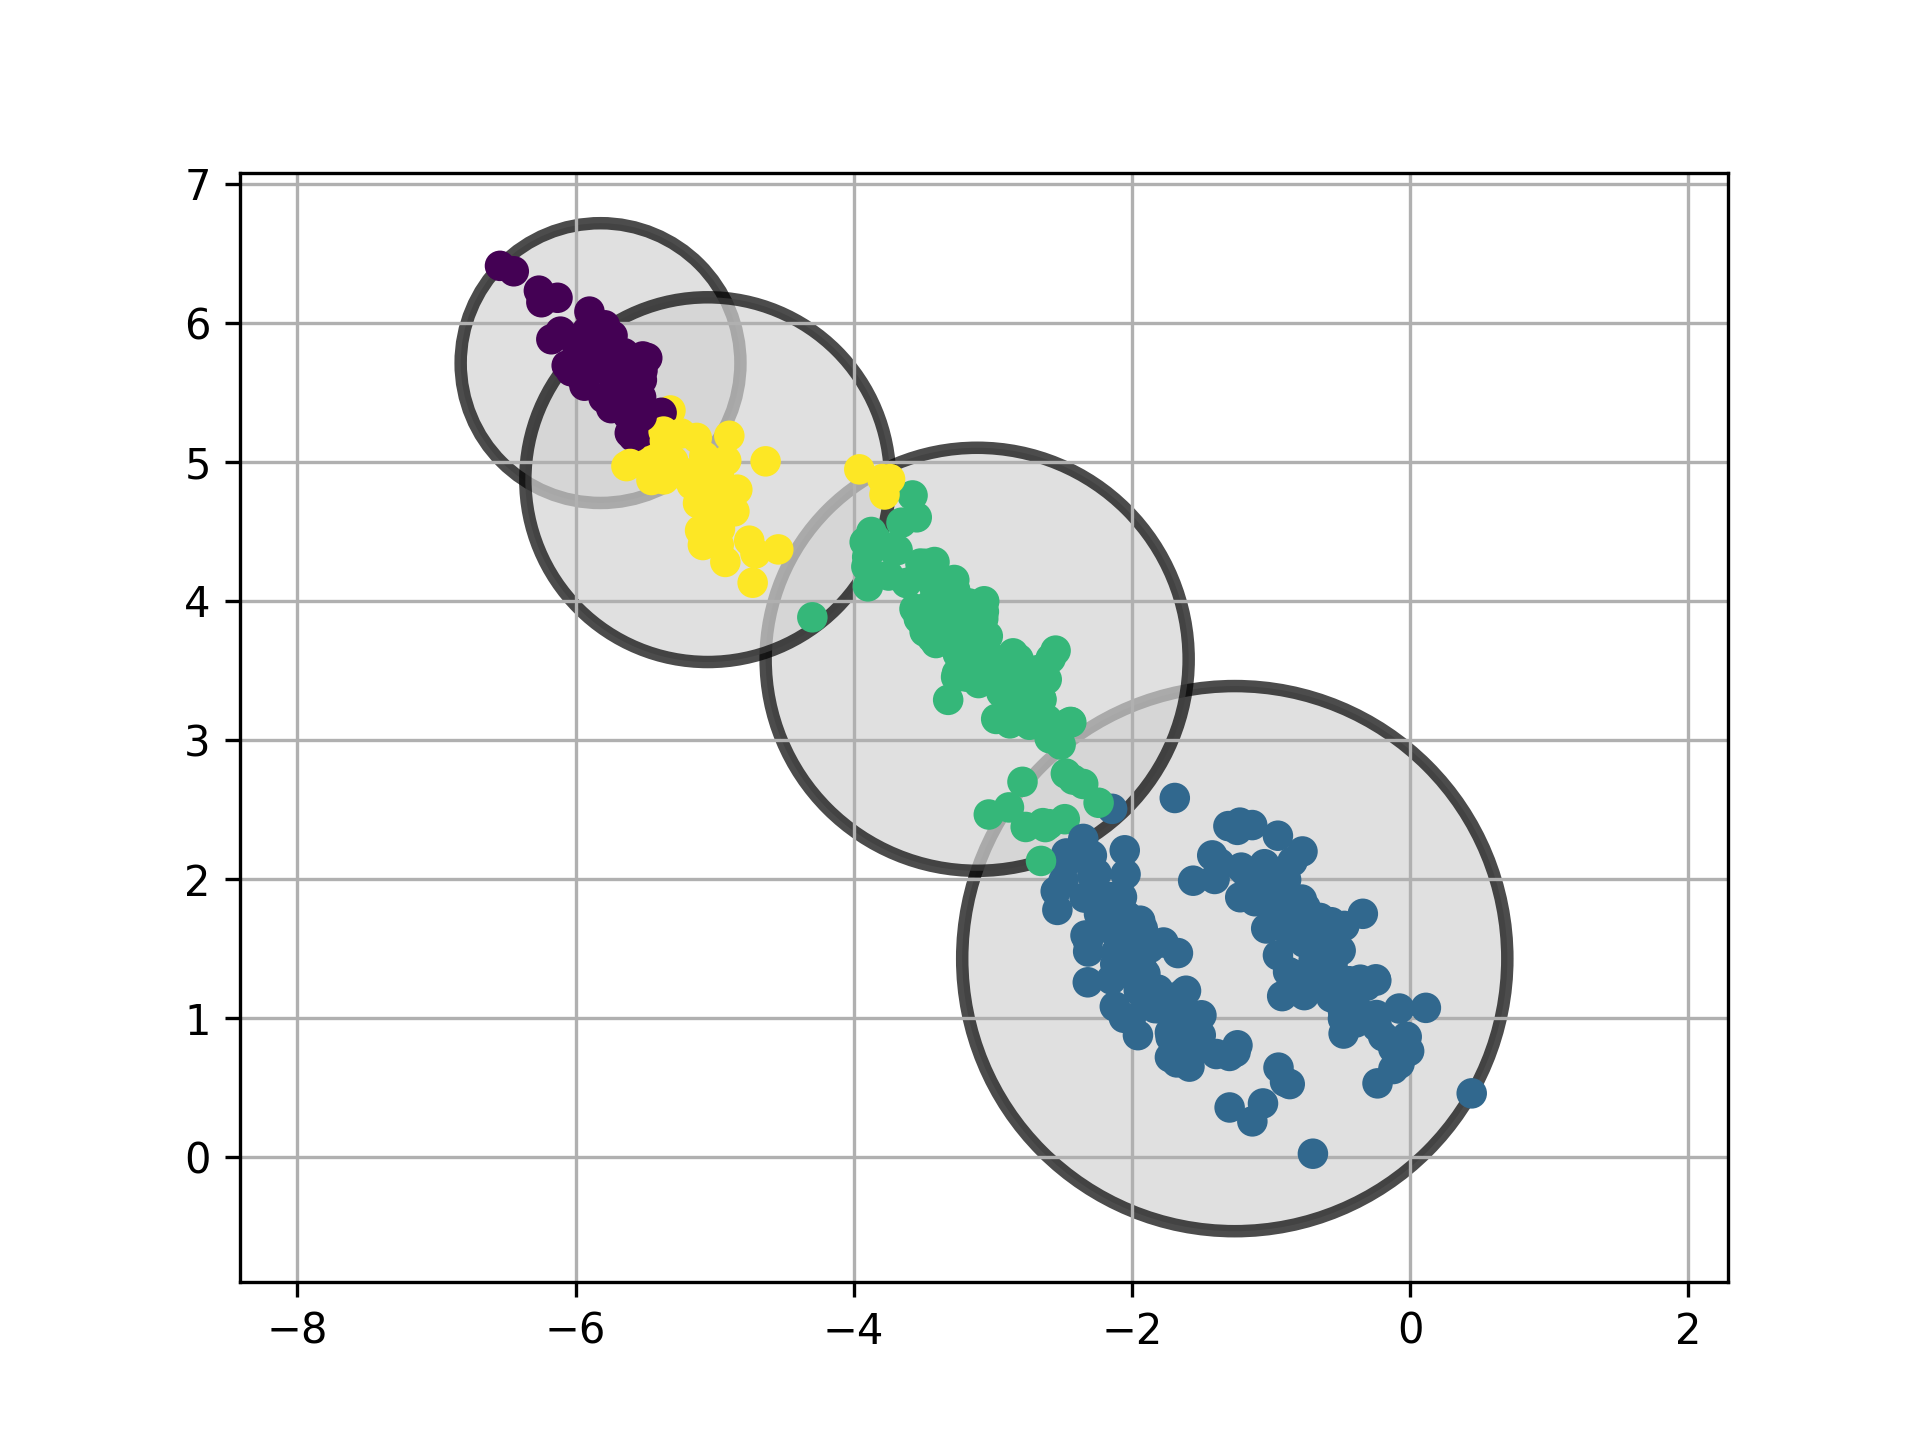
\includegraphics[width=\textwidth]{../img/fig48-3.png}
        \caption{Poor performance of k-means for noncircular clusters}
    \end{subfigure}
    \caption{Motivating Gaussian Mixtures: Weaknesses of k-Means}
\end{figure}

These two disadvantages of k-means—its \important{lack of flexibility in cluster shape and lack of probabilistic cluster assignment}—mean that for many datasets (especially low-dimensional datasets) it may not perform as well as you might hope.

\section{Generalizing E–M: Gaussian Mixture Models}
A \textbf{Gaussian mixture model} (GMM) attempts to find a mixture of multidimensional
Gaussian probability distributions that best model any input dataset.

Under the hood, a Gaussian mixture model is very similar to k-means: it uses an
expectation–maximization approach, which qualitatively does the following:
\begin{enumerate}
    \item Choose starting guesses for the location and shape.
    \item Repeat until converged:
          \begin{enumerate}
              \item E-step: For each point, find weights encoding the probability of membership in each cluster.
              \item M-step: For each cluster, update its location, normalization, and shape based on all data points, making use of the weights.
          \end{enumerate}
\end{enumerate}
The result of this is that each cluster is associated not with a hard-edged sphere, but
with a smooth Gaussian model. Just as in the k-means expectation–maximization
approach, this algorithm can sometimes miss the globally optimal solution, and thus
in practice multiple random initializations are used.

\section{Choosing the Covariance Type}
If you look at the details of the preceding fits, you will see that the \verb|covariance_type| option was set differently within each. This hyperparameter controls the degrees of freedom in the shape of each cluster; it's essential to set this carefully for any given problem. The default is \verb|covariance_type="diag"|, which means that the size of the cluster along each dimension can be set independently, with the resulting ellipse constrained to align with the axes. \verb|covariance_type="spherical"| is a slightly simpler and faster model, which constrains the shape of the cluster such that all dimensions
are equal. The resulting clustering will have similar characteristics to that of k-means,
though it's not entirely equivalent. A more complicated and computationally expensive model (especially as the number of dimensions grows) is to use \verb|covariance_type="full"|, which allows each cluster to be modeled as an ellipse with arbitrary orientation.

\section{Gaussian Mixture Models as Density Estimation}
Though the GMM is often categorized as a clustering algorithm, fundamentally it is an algorithm for density estimation. That is to say, the result of a GMM fit to some data is technically not a clustering model, but a generative probabilistic model describing the distribution of the data.

A GMM is convenient as a flexible means of modeling an arbitrary multidimensional
distribution of data.
The fact that a GMM is a generative model gives us a natural means of determining
the optimal number of components for a given dataset. A generative model is inherently a probability distribution for the dataset, and so we can simply evaluate the likelihood of the data under the model, using cross-validation to avoid overfitting.
Another means of correcting for overfitting is to adjust the model likelihoods using
some analytic criterion such as the \href{https://en.wikipedia.org/wiki/Akaike_information_criterion}{Akaike information criterion (AIC)} or \href{https://en.wikipedia.org/wiki/Bayesian_information_criterion}{the Bayesian information criterion (BIC)}.